\documentclass[twoside]{book}

% Packages required by doxygen
\usepackage{fixltx2e}
\usepackage{calc}
\usepackage{doxygen}
\usepackage{graphicx}
\usepackage[utf8]{inputenc}
\usepackage{makeidx}
\usepackage{multicol}
\usepackage{multirow}
\PassOptionsToPackage{warn}{textcomp}
\usepackage{textcomp}
\usepackage[nointegrals]{wasysym}
\usepackage[table]{xcolor}

% Font selection
\usepackage[T1]{fontenc}
\usepackage{mathptmx}
\usepackage[scaled=.90]{helvet}
\usepackage{courier}
\usepackage{amssymb}
\usepackage{sectsty}
\renewcommand{\familydefault}{\sfdefault}
\allsectionsfont{%
  \fontseries{bc}\selectfont%
  \color{darkgray}%
}
\renewcommand{\DoxyLabelFont}{%
  \fontseries{bc}\selectfont%
  \color{darkgray}%
}
\newcommand{\+}{\discretionary{\mbox{\scriptsize$\hookleftarrow$}}{}{}}

% Page & text layout
\usepackage{geometry}
\geometry{%
  a4paper,%
  top=2.5cm,%
  bottom=2.5cm,%
  left=2.5cm,%
  right=2.5cm%
}
\tolerance=750
\hfuzz=15pt
\hbadness=750
\setlength{\emergencystretch}{15pt}
\setlength{\parindent}{0cm}
\setlength{\parskip}{0.2cm}
\makeatletter
\renewcommand{\paragraph}{%
  \@startsection{paragraph}{4}{0ex}{-1.0ex}{1.0ex}{%
    \normalfont\normalsize\bfseries\SS@parafont%
  }%
}
\renewcommand{\subparagraph}{%
  \@startsection{subparagraph}{5}{0ex}{-1.0ex}{1.0ex}{%
    \normalfont\normalsize\bfseries\SS@subparafont%
  }%
}
\makeatother

% Headers & footers
\usepackage{fancyhdr}
\pagestyle{fancyplain}
\fancyhead[LE]{\fancyplain{}{\bfseries\thepage}}
\fancyhead[CE]{\fancyplain{}{}}
\fancyhead[RE]{\fancyplain{}{\bfseries\leftmark}}
\fancyhead[LO]{\fancyplain{}{\bfseries\rightmark}}
\fancyhead[CO]{\fancyplain{}{}}
\fancyhead[RO]{\fancyplain{}{\bfseries\thepage}}
\fancyfoot[LE]{\fancyplain{}{}}
\fancyfoot[CE]{\fancyplain{}{}}
\fancyfoot[RE]{\fancyplain{}{\bfseries\scriptsize Generated on Sun Jan 11 2015 20\+:34\+:21 for ws2 by Doxygen }}
\fancyfoot[LO]{\fancyplain{}{\bfseries\scriptsize Generated on Sun Jan 11 2015 20\+:34\+:21 for ws2 by Doxygen }}
\fancyfoot[CO]{\fancyplain{}{}}
\fancyfoot[RO]{\fancyplain{}{}}
\renewcommand{\footrulewidth}{0.4pt}
\renewcommand{\chaptermark}[1]{%
  \markboth{#1}{}%
}
\renewcommand{\sectionmark}[1]{%
  \markright{\thesection\ #1}%
}

% Indices & bibliography
\usepackage{natbib}
\usepackage[titles]{tocloft}
\setcounter{tocdepth}{3}
\setcounter{secnumdepth}{5}
\makeindex

% Hyperlinks (required, but should be loaded last)
\usepackage{ifpdf}
\ifpdf
  \usepackage[pdftex,pagebackref=true]{hyperref}
\else
  \usepackage[ps2pdf,pagebackref=true]{hyperref}
\fi
\hypersetup{%
  colorlinks=true,%
  linkcolor=blue,%
  citecolor=blue,%
  unicode%
}

% Custom commands
\newcommand{\clearemptydoublepage}{%
  \newpage{\pagestyle{empty}\cleardoublepage}%
}


%===== C O N T E N T S =====

\begin{document}

% Titlepage & ToC
\hypersetup{pageanchor=false,
             bookmarks=true,
             bookmarksnumbered=true,
             pdfencoding=unicode
            }
\pagenumbering{roman}
\begin{titlepage}
\vspace*{7cm}
\begin{center}%
{\Large ws2 }\\
\vspace*{1cm}
{\large Generated by Doxygen 1.8.8}\\
\vspace*{0.5cm}
{\small Sun Jan 11 2015 20:34:21}\\
\end{center}
\end{titlepage}
\clearemptydoublepage
\tableofcontents
\clearemptydoublepage
\pagenumbering{arabic}
\hypersetup{pageanchor=true}

%--- Begin generated contents ---
\chapter{Namespace Index}
\section{Namespace List}
Here is a list of all documented namespaces with brief descriptions\+:\begin{DoxyCompactList}
\item\contentsline{section}{\hyperlink{namespace_w_s2}{W\+S2} }{\pageref{namespace_w_s2}}{}
\end{DoxyCompactList}

\chapter{Hierarchical Index}
\section{Class Hierarchy}
This inheritance list is sorted roughly, but not completely, alphabetically\+:\begin{DoxyCompactList}
\item \contentsline{section}{php}{\pageref{class_1_1_authorization_1_1php}}{}
\item \contentsline{section}{php}{\pageref{class_1_1_caretaker_1_1php}}{}
\item \contentsline{section}{php}{\pageref{class_1_1_user_1_1php}}{}
\item \contentsline{section}{php}{\pageref{class_1_1_pacient_1_1php}}{}
\item \contentsline{section}{php}{\pageref{class_1_1_pacient_info_1_1php}}{}
\item \contentsline{section}{php}{\pageref{class_1_1_webservice_1_1php}}{}
\item \contentsline{section}{W\+S2\+\_\+\+Authorization}{\pageref{class_w_s2___authorization}}{}
\item \contentsline{section}{W\+S2\+\_\+\+Pacient\+Info}{\pageref{class_w_s2___pacient_info}}{}
\item \contentsline{section}{W\+S2\+\_\+\+User}{\pageref{class_w_s2___user}}{}
\begin{DoxyCompactList}
\item \contentsline{section}{W\+S2\+\_\+\+Caretaker}{\pageref{class_w_s2___caretaker}}{}
\item \contentsline{section}{W\+S2\+\_\+\+Pacient}{\pageref{class_w_s2___pacient}}{}
\end{DoxyCompactList}
\item \contentsline{section}{W\+S2\+\_\+\+Webservice}{\pageref{class_w_s2___webservice}}{}
\end{DoxyCompactList}

\chapter{Data Structure Index}
\section{Data Structures}
Here are the data structures with brief descriptions\+:\begin{DoxyCompactList}
\item\contentsline{section}{\hyperlink{class_1_1_authorization_1_1php}{php} }{\pageref{class_1_1_authorization_1_1php}}{}
\item\contentsline{section}{\hyperlink{class_1_1_caretaker_1_1php}{php} }{\pageref{class_1_1_caretaker_1_1php}}{}
\item\contentsline{section}{\hyperlink{class_1_1_user_1_1php}{php} }{\pageref{class_1_1_user_1_1php}}{}
\item\contentsline{section}{\hyperlink{class_1_1_pacient_1_1php}{php} }{\pageref{class_1_1_pacient_1_1php}}{}
\item\contentsline{section}{\hyperlink{class_1_1_pacient_info_1_1php}{php} }{\pageref{class_1_1_pacient_info_1_1php}}{}
\item\contentsline{section}{\hyperlink{class_1_1_webservice_1_1php}{php} }{\pageref{class_1_1_webservice_1_1php}}{}
\item\contentsline{section}{\hyperlink{class_w_s2___authorization}{W\+S2\+\_\+\+Authorization} }{\pageref{class_w_s2___authorization}}{}
\item\contentsline{section}{\hyperlink{class_w_s2___caretaker}{W\+S2\+\_\+\+Caretaker} }{\pageref{class_w_s2___caretaker}}{}
\item\contentsline{section}{\hyperlink{class_w_s2___pacient}{W\+S2\+\_\+\+Pacient} }{\pageref{class_w_s2___pacient}}{}
\item\contentsline{section}{\hyperlink{class_w_s2___pacient_info}{W\+S2\+\_\+\+Pacient\+Info} }{\pageref{class_w_s2___pacient_info}}{}
\item\contentsline{section}{\hyperlink{class_w_s2___user}{W\+S2\+\_\+\+User} }{\pageref{class_w_s2___user}}{}
\item\contentsline{section}{\hyperlink{class_w_s2___webservice}{W\+S2\+\_\+\+Webservice} }{\pageref{class_w_s2___webservice}}{}
\end{DoxyCompactList}

\chapter{Namespace Documentation}
\hypertarget{namespace_w_s2}{\section{W\+S2 Namespace Reference}
\label{namespace_w_s2}\index{W\+S2@{W\+S2}}
}


\subsection{Detailed Description}
include \hyperlink{class_w_s2___pacient_info}{W\+S2\+\_\+\+Pacient\+Info}

\begin{DoxyAuthor}{Author}
firstname and lastname of author, \href{mailto:author@example.org}{\tt author@example.\+org} link a given caretaker to a pacient activity into the database
\end{DoxyAuthor}
public \begin{DoxyAuthor}{Author}
firstname and lastname of author, \href{mailto:author@example.org}{\tt author@example.\+org}
\end{DoxyAuthor}
Short description of class \hyperlink{class_w_s2___caretaker}{W\+S2\+\_\+\+Caretaker}

public \begin{DoxyAuthor}{Author}
firstname and lastname of author, \href{mailto:author@example.org}{\tt author@example.\+org}
\end{DoxyAuthor}
Short description of class \hyperlink{class_w_s2___pacient}{W\+S2\+\_\+\+Pacient}

public \begin{DoxyAuthor}{Author}
firstname and lastname of author, \href{mailto:author@example.org}{\tt author@example.\+org}
\end{DoxyAuthor}
stores an the url of an activity of a pacient

public \begin{DoxyAuthor}{Author}
firstname and lastname of author, \href{mailto:author@example.org}{\tt author@example.\+org}
\end{DoxyAuthor}
a generic user for the webservice 2

public \begin{DoxyAuthor}{Author}
firstname and lastname of author, \href{mailto:author@example.org}{\tt author@example.\+org}
\end{DoxyAuthor}
include \hyperlink{class_w_s2___pacient}{W\+S2\+\_\+\+Pacient}

\begin{DoxyAuthor}{Author}
firstname and lastname of author, \href{mailto:author@example.org}{\tt author@example.\+org} include \hyperlink{class_w_s2___pacient_info}{W\+S2\+\_\+\+Pacient\+Info}

firstname and lastname of author, \href{mailto:author@example.org}{\tt author@example.\+org} Short description of class \hyperlink{class_w_s2___webservice}{W\+S2\+\_\+\+Webservice}
\end{DoxyAuthor}
public \begin{DoxyAuthor}{Author}
firstname and lastname of author, \href{mailto:author@example.org}{\tt author@example.\+org} 
\end{DoxyAuthor}

\chapter{Data Structure Documentation}
\hypertarget{class_1_1_authorization_1_1php}{\section{php Class Reference}
\label{class_1_1_authorization_1_1php}\index{php@{php}}
}


\subsection{Detailed Description}
S\+E-\/\+Project -\/ \hyperlink{namespace_w_s2}{W\+S2}

\$\+Id\$

This file is part of S\+E-\/\+Project.

Automatically generated on 09.\+01.\+2015, 14\+:55\+:15 with Argo\+U\+M\+L P\+H\+P module (last revised \begin{DoxyParagraph}{Date}
2010-\/01-\/12 20\+:14\+:42 +0100 (Tue, 12 Jan 2010) 
\end{DoxyParagraph}
)

\begin{DoxyAuthor}{Author}
firstname and lastname of author, \href{mailto:author@example.org}{\tt author@example.\+org} 
\end{DoxyAuthor}


The documentation for this class was generated from the following file\+:\begin{DoxyCompactItemize}
\item 
C\+:/\+Users/\+Alessandro/\+Desktop/\+E\+S-\/\+Project/\+W\+S2/class.\+Authorization.\+php\end{DoxyCompactItemize}

\hypertarget{class_1_1_caretaker_1_1php}{\section{php Class Reference}
\label{class_1_1_caretaker_1_1php}\index{php@{php}}
}


\subsection{Detailed Description}
S\+E-\/\+Project -\/ \hyperlink{namespace_w_s2}{W\+S2}

\$\+Id\$

This file is part of S\+E-\/\+Project.

Automatically generated on 07.\+01.\+2015, 17\+:09\+:54 with Argo\+U\+M\+L P\+H\+P module (last revised \begin{DoxyParagraph}{Date}
2010-\/01-\/12 20\+:14\+:42 +0100 (Tue, 12 Jan 2010) 
\end{DoxyParagraph}
)

\begin{DoxyAuthor}{Author}
firstname and lastname of author, \href{mailto:author@example.org}{\tt author@example.\+org} 
\end{DoxyAuthor}


The documentation for this class was generated from the following file\+:\begin{DoxyCompactItemize}
\item 
C\+:/\+Users/\+Alessandro/\+Desktop/\+E\+S-\/\+Project/\+W\+S2/class.\+Caretaker.\+php\end{DoxyCompactItemize}

\hypertarget{class_1_1_user_1_1php}{\section{php Class Reference}
\label{class_1_1_user_1_1php}\index{php@{php}}
}


\subsection{Detailed Description}
S\+E-\/\+Project -\/ \hyperlink{namespace_w_s2}{W\+S2}

\$\+Id\$

This file is part of S\+E-\/\+Project.

Automatically generated on 07.\+01.\+2015, 17\+:09\+:54 with Argo\+U\+M\+L P\+H\+P module (last revised \begin{DoxyParagraph}{Date}
2010-\/01-\/12 20\+:14\+:42 +0100 (Tue, 12 Jan 2010) 
\end{DoxyParagraph}
)

\begin{DoxyAuthor}{Author}
firstname and lastname of author, \href{mailto:author@example.org}{\tt author@example.\+org} 
\end{DoxyAuthor}


The documentation for this class was generated from the following file\+:\begin{DoxyCompactItemize}
\item 
C\+:/\+Users/\+Alessandro/\+Desktop/\+E\+S-\/\+Project/\+W\+S2/class.\+User.\+php\end{DoxyCompactItemize}

\hypertarget{class_1_1_pacient_1_1php}{\section{php Class Reference}
\label{class_1_1_pacient_1_1php}\index{php@{php}}
}


\subsection{Detailed Description}
S\+E-\/\+Project -\/ \hyperlink{namespace_w_s2}{W\+S2}

\$\+Id\$

This file is part of S\+E-\/\+Project.

Automatically generated on 07.\+01.\+2015, 17\+:09\+:54 with Argo\+U\+M\+L P\+H\+P module (last revised \begin{DoxyParagraph}{Date}
2010-\/01-\/12 20\+:14\+:42 +0100 (Tue, 12 Jan 2010) 
\end{DoxyParagraph}
)

\begin{DoxyAuthor}{Author}
firstname and lastname of author, \href{mailto:author@example.org}{\tt author@example.\+org} 
\end{DoxyAuthor}


The documentation for this class was generated from the following file\+:\begin{DoxyCompactItemize}
\item 
C\+:/\+Users/\+Alessandro/\+Desktop/\+E\+S-\/\+Project/\+W\+S2/class.\+Pacient.\+php\end{DoxyCompactItemize}

\hypertarget{class_1_1_pacient_info_1_1php}{\section{php Class Reference}
\label{class_1_1_pacient_info_1_1php}\index{php@{php}}
}


\subsection{Detailed Description}
S\+E-\/\+Project -\/ \hyperlink{namespace_w_s2}{W\+S2}

\$\+Id\$

This file is part of S\+E-\/\+Project.

Automatically generated on 07.\+01.\+2015, 17\+:09\+:54 with Argo\+U\+M\+L P\+H\+P module (last revised \begin{DoxyParagraph}{Date}
2010-\/01-\/12 20\+:14\+:42 +0100 (Tue, 12 Jan 2010) 
\end{DoxyParagraph}
)

\begin{DoxyAuthor}{Author}
firstname and lastname of author, \href{mailto:author@example.org}{\tt author@example.\+org} 
\end{DoxyAuthor}


The documentation for this class was generated from the following file\+:\begin{DoxyCompactItemize}
\item 
C\+:/\+Users/\+Alessandro/\+Desktop/\+E\+S-\/\+Project/\+W\+S2/class.\+Pacient\+Info.\+php\end{DoxyCompactItemize}

\hypertarget{class_1_1_webservice_1_1php}{\section{php Class Reference}
\label{class_1_1_webservice_1_1php}\index{php@{php}}
}


\subsection{Detailed Description}
S\+E-\/\+Project -\/ \hyperlink{namespace_w_s2}{W\+S2}

\$\+Id\$

This file is part of S\+E-\/\+Project.

Automatically generated on 07.\+01.\+2015, 17\+:09\+:54 with Argo\+U\+M\+L P\+H\+P module (last revised \begin{DoxyParagraph}{Date}
2010-\/01-\/12 20\+:14\+:42 +0100 (Tue, 12 Jan 2010) 
\end{DoxyParagraph}
)

\begin{DoxyAuthor}{Author}
firstname and lastname of author, \href{mailto:author@example.org}{\tt author@example.\+org} 
\end{DoxyAuthor}


The documentation for this class was generated from the following file\+:\begin{DoxyCompactItemize}
\item 
C\+:/\+Users/\+Alessandro/\+Desktop/\+E\+S-\/\+Project/\+W\+S2/class.\+Webservice.\+php\end{DoxyCompactItemize}

\hypertarget{class_w_s2___authorization}{\section{W\+S2\+\_\+\+Authorization Class Reference}
\label{class_w_s2___authorization}\index{W\+S2\+\_\+\+Authorization@{W\+S2\+\_\+\+Authorization}}
}
\subsection*{Public Member Functions}
\begin{DoxyCompactItemize}
\item 
\hypertarget{class_w_s2___authorization_ac2158e32a66541df88687210ec8fa1e5}{{\bfseries get\+Pacient\+Info\+Id} ()}\label{class_w_s2___authorization_ac2158e32a66541df88687210ec8fa1e5}

\item 
\hypertarget{class_w_s2___authorization_a686e842b224af6da713dd6437c9c9b7a}{{\bfseries get\+Caretaker} ()}\label{class_w_s2___authorization_a686e842b224af6da713dd6437c9c9b7a}

\end{DoxyCompactItemize}
\subsection*{Static Public Member Functions}
\begin{DoxyCompactItemize}
\item 
static \hyperlink{class_w_s2___authorization_a279b221e07fd283920ebfb16ca8b3be0}{authorize\+Caretaker} (\$caretaker, \$pacient\+Info)
\item 
static \hyperlink{class_w_s2___authorization_a9a173416a1ed7d16e09512827febecc8}{is\+Caretaker\+Authorized} (\$pacient\+Info, \$caretaker)
\end{DoxyCompactItemize}


\subsection{Member Function Documentation}
\hypertarget{class_w_s2___authorization_a279b221e07fd283920ebfb16ca8b3be0}{\index{W\+S2\+\_\+\+Authorization@{W\+S2\+\_\+\+Authorization}!authorize\+Caretaker@{authorize\+Caretaker}}
\index{authorize\+Caretaker@{authorize\+Caretaker}!W\+S2\+\_\+\+Authorization@{W\+S2\+\_\+\+Authorization}}
\subsubsection[{authorize\+Caretaker}]{\setlength{\rightskip}{0pt plus 5cm}static authorize\+Caretaker (
\begin{DoxyParamCaption}
\item[{}]{\$caretaker, }
\item[{}]{\$pacient\+Info}
\end{DoxyParamCaption}
)\hspace{0.3cm}{\ttfamily [static]}}}\label{class_w_s2___authorization_a279b221e07fd283920ebfb16ca8b3be0}
authorize a caretaker to have access to a pacient activity

\begin{DoxyAuthor}{Author}
firstname and lastname of author, \href{mailto:author@example.org}{\tt author@example.\+org} 
\end{DoxyAuthor}

\begin{DoxyParams}{Parameters}
{\em String} & caretaker \\
\hline
{\em Integer} & pacient\+Info return String \\
\hline
\end{DoxyParams}
\hypertarget{class_w_s2___authorization_a9a173416a1ed7d16e09512827febecc8}{\index{W\+S2\+\_\+\+Authorization@{W\+S2\+\_\+\+Authorization}!is\+Caretaker\+Authorized@{is\+Caretaker\+Authorized}}
\index{is\+Caretaker\+Authorized@{is\+Caretaker\+Authorized}!W\+S2\+\_\+\+Authorization@{W\+S2\+\_\+\+Authorization}}
\subsubsection[{is\+Caretaker\+Authorized}]{\setlength{\rightskip}{0pt plus 5cm}static is\+Caretaker\+Authorized (
\begin{DoxyParamCaption}
\item[{}]{\$pacient\+Info, }
\item[{}]{\$caretaker}
\end{DoxyParamCaption}
)\hspace{0.3cm}{\ttfamily [static]}}}\label{class_w_s2___authorization_a9a173416a1ed7d16e09512827febecc8}
check if a caretaker is authorized to access a pacient activity

\begin{DoxyAuthor}{Author}
firstname and lastname of author, \href{mailto:author@example.org}{\tt author@example.\+org} 
\end{DoxyAuthor}

\begin{DoxyParams}{Parameters}
{\em String} & caretaker \\
\hline
{\em Integer} & pacient\+Info return String \\
\hline
\end{DoxyParams}


The documentation for this class was generated from the following file\+:\begin{DoxyCompactItemize}
\item 
C\+:/\+Users/\+Alessandro/\+Desktop/\+E\+S-\/\+Project/\+W\+S2/class.\+Authorization.\+php\end{DoxyCompactItemize}

\hypertarget{class_w_s2___caretaker}{\section{W\+S2\+\_\+\+Caretaker Class Reference}
\label{class_w_s2___caretaker}\index{W\+S2\+\_\+\+Caretaker@{W\+S2\+\_\+\+Caretaker}}
}
Inheritance diagram for W\+S2\+\_\+\+Caretaker\+:\begin{figure}[H]
\begin{center}
\leavevmode
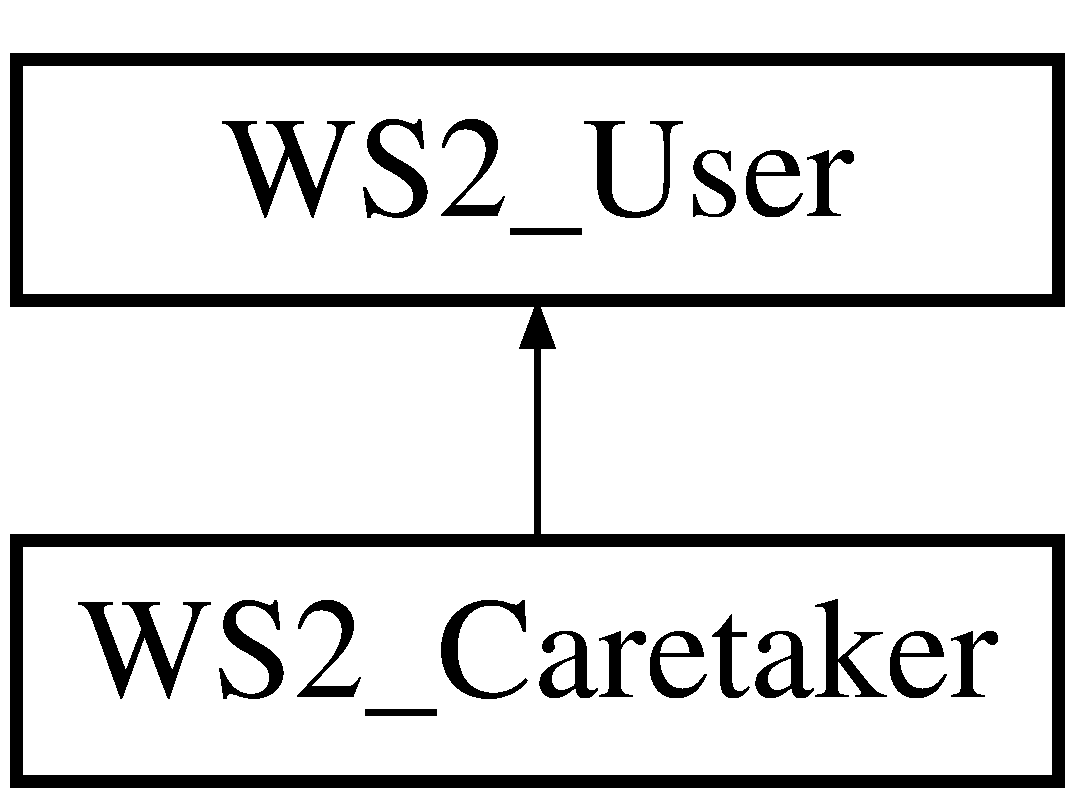
\includegraphics[height=2.000000cm]{class_w_s2___caretaker}
\end{center}
\end{figure}
\subsection*{Public Member Functions}
\begin{DoxyCompactItemize}
\item 
\hypertarget{class_w_s2___caretaker_a42c9621713b6dcdfb9edd5a7630b6d93}{{\bfseries get\+Firstname} ()}\label{class_w_s2___caretaker_a42c9621713b6dcdfb9edd5a7630b6d93}

\item 
\hypertarget{class_w_s2___caretaker_a5d606fdf02d35b79b74b91a88c09000f}{{\bfseries get\+Lastname} ()}\label{class_w_s2___caretaker_a5d606fdf02d35b79b74b91a88c09000f}

\item 
\hypertarget{class_w_s2___caretaker_a81b37a3c9d639574e394f80c1138c75e}{{\bfseries get\+Username} ()}\label{class_w_s2___caretaker_a81b37a3c9d639574e394f80c1138c75e}

\item 
\hypertarget{class_w_s2___caretaker_aeafdb95ad7b97a5ff68ac785e8c243e5}{{\bfseries get\+Birthdate} ()}\label{class_w_s2___caretaker_aeafdb95ad7b97a5ff68ac785e8c243e5}

\item 
\hypertarget{class_w_s2___caretaker_af7313369f22d5c761e16462abe0c6ae1}{{\bfseries get\+Gender} ()}\label{class_w_s2___caretaker_af7313369f22d5c761e16462abe0c6ae1}

\item 
\hypertarget{class_w_s2___caretaker_a211a2979c22afcd7d9056a2bb55aa449}{{\bfseries get\+Token} ()}\label{class_w_s2___caretaker_a211a2979c22afcd7d9056a2bb55aa449}

\item 
\hyperlink{class_w_s2___caretaker_a471f3c30d6c985670b14543252f47ab0}{register\+Caretaker} ()
\end{DoxyCompactItemize}
\subsection*{Static Public Member Functions}
\begin{DoxyCompactItemize}
\item 
static \hyperlink{class_w_s2___caretaker_ae218ade97397832878ac6b5758036632}{exist\+Caretaker} (\$caretaker)
\end{DoxyCompactItemize}


\subsection{Member Function Documentation}
\hypertarget{class_w_s2___caretaker_ae218ade97397832878ac6b5758036632}{\index{W\+S2\+\_\+\+Caretaker@{W\+S2\+\_\+\+Caretaker}!exist\+Caretaker@{exist\+Caretaker}}
\index{exist\+Caretaker@{exist\+Caretaker}!W\+S2\+\_\+\+Caretaker@{W\+S2\+\_\+\+Caretaker}}
\subsubsection[{exist\+Caretaker}]{\setlength{\rightskip}{0pt plus 5cm}static exist\+Caretaker (
\begin{DoxyParamCaption}
\item[{}]{\$caretaker}
\end{DoxyParamCaption}
)\hspace{0.3cm}{\ttfamily [static]}}}\label{class_w_s2___caretaker_ae218ade97397832878ac6b5758036632}
check if a given caretaker is in the database

\begin{DoxyAuthor}{Author}
firstname and lastname of author, \href{mailto:author@example.org}{\tt author@example.\+org} 
\end{DoxyAuthor}

\begin{DoxyParams}{Parameters}
{\em String} & caretaker return boolean \\
\hline
\end{DoxyParams}
\hypertarget{class_w_s2___caretaker_a471f3c30d6c985670b14543252f47ab0}{\index{W\+S2\+\_\+\+Caretaker@{W\+S2\+\_\+\+Caretaker}!register\+Caretaker@{register\+Caretaker}}
\index{register\+Caretaker@{register\+Caretaker}!W\+S2\+\_\+\+Caretaker@{W\+S2\+\_\+\+Caretaker}}
\subsubsection[{register\+Caretaker}]{\setlength{\rightskip}{0pt plus 5cm}register\+Caretaker (
\begin{DoxyParamCaption}
{}
\end{DoxyParamCaption}
)}}\label{class_w_s2___caretaker_a471f3c30d6c985670b14543252f47ab0}
register a caretaker into the ws2 database

\begin{DoxyAuthor}{Author}
firstname and lastname of author, \href{mailto:author@example.org}{\tt author@example.\+org} return String 
\end{DoxyAuthor}


The documentation for this class was generated from the following file\+:\begin{DoxyCompactItemize}
\item 
C\+:/\+Users/\+Alessandro/\+Desktop/\+E\+S-\/\+Project/\+W\+S2/class.\+Caretaker.\+php\end{DoxyCompactItemize}

\hypertarget{class_w_s2___pacient}{\section{W\+S2\+\_\+\+Pacient Class Reference}
\label{class_w_s2___pacient}\index{W\+S2\+\_\+\+Pacient@{W\+S2\+\_\+\+Pacient}}
}
Inheritance diagram for W\+S2\+\_\+\+Pacient\+:\begin{figure}[H]
\begin{center}
\leavevmode
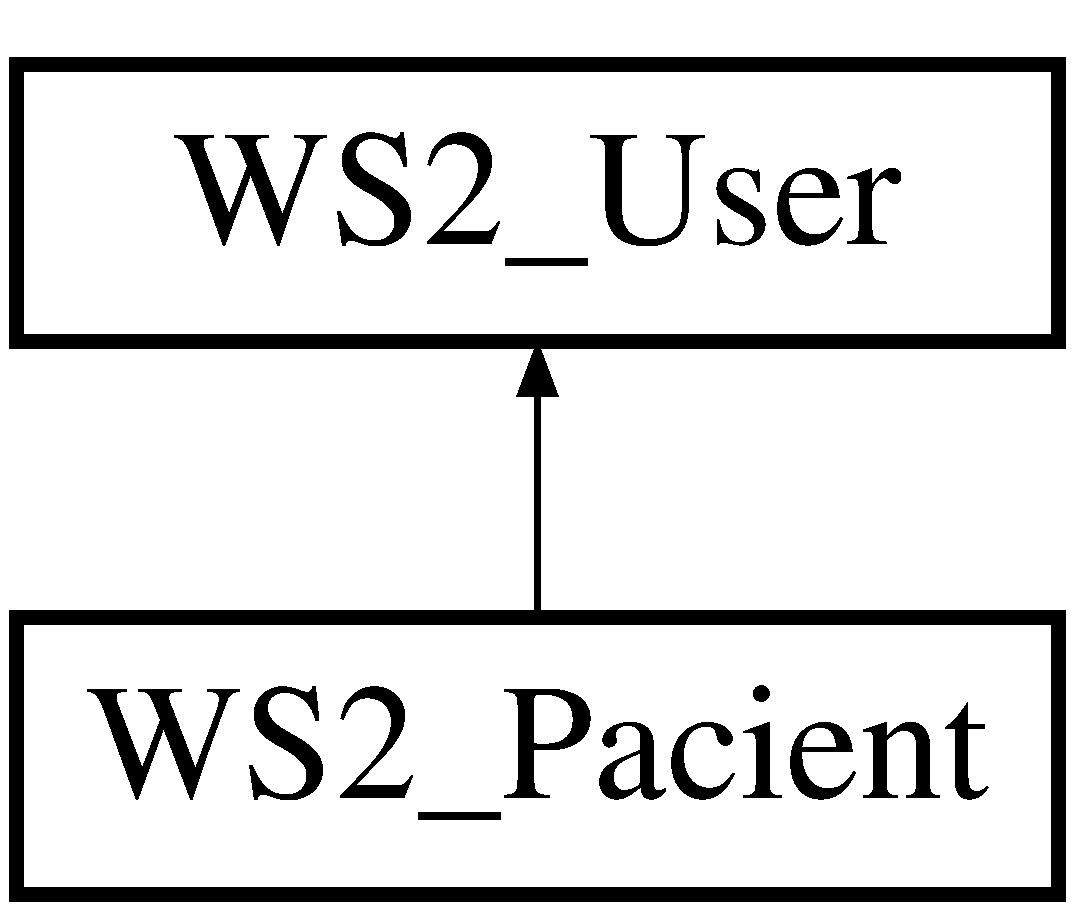
\includegraphics[height=2.000000cm]{class_w_s2___pacient}
\end{center}
\end{figure}
\subsection*{Public Member Functions}
\begin{DoxyCompactItemize}
\item 
\hypertarget{class_w_s2___pacient_a42c9621713b6dcdfb9edd5a7630b6d93}{{\bfseries get\+Firstname} ()}\label{class_w_s2___pacient_a42c9621713b6dcdfb9edd5a7630b6d93}

\item 
\hypertarget{class_w_s2___pacient_a5d606fdf02d35b79b74b91a88c09000f}{{\bfseries get\+Lastname} ()}\label{class_w_s2___pacient_a5d606fdf02d35b79b74b91a88c09000f}

\item 
\hypertarget{class_w_s2___pacient_a81b37a3c9d639574e394f80c1138c75e}{{\bfseries get\+Username} ()}\label{class_w_s2___pacient_a81b37a3c9d639574e394f80c1138c75e}

\item 
\hypertarget{class_w_s2___pacient_aeafdb95ad7b97a5ff68ac785e8c243e5}{{\bfseries get\+Birthdate} ()}\label{class_w_s2___pacient_aeafdb95ad7b97a5ff68ac785e8c243e5}

\item 
\hypertarget{class_w_s2___pacient_af7313369f22d5c761e16462abe0c6ae1}{{\bfseries get\+Gender} ()}\label{class_w_s2___pacient_af7313369f22d5c761e16462abe0c6ae1}

\item 
\hypertarget{class_w_s2___pacient_a211a2979c22afcd7d9056a2bb55aa449}{{\bfseries get\+Token} ()}\label{class_w_s2___pacient_a211a2979c22afcd7d9056a2bb55aa449}

\item 
\hyperlink{class_w_s2___pacient_a46300e082e774bfcef7b063ea442cf77}{register\+Pacient} ()
\end{DoxyCompactItemize}
\subsection*{Static Public Member Functions}
\begin{DoxyCompactItemize}
\item 
static \hyperlink{class_w_s2___pacient_a07a6e01f4de7bc49344ec16dbaaa5722}{exist\+Pacient} (\$pacient)
\item 
static \hyperlink{class_w_s2___pacient_ac8852c86222d7ee44ae459d779d560dd}{validate\+Pacient} (\$pacient, \$token)
\end{DoxyCompactItemize}


\subsection{Member Function Documentation}
\hypertarget{class_w_s2___pacient_a07a6e01f4de7bc49344ec16dbaaa5722}{\index{W\+S2\+\_\+\+Pacient@{W\+S2\+\_\+\+Pacient}!exist\+Pacient@{exist\+Pacient}}
\index{exist\+Pacient@{exist\+Pacient}!W\+S2\+\_\+\+Pacient@{W\+S2\+\_\+\+Pacient}}
\subsubsection[{exist\+Pacient}]{\setlength{\rightskip}{0pt plus 5cm}static exist\+Pacient (
\begin{DoxyParamCaption}
\item[{}]{\$pacient}
\end{DoxyParamCaption}
)\hspace{0.3cm}{\ttfamily [static]}}}\label{class_w_s2___pacient_a07a6e01f4de7bc49344ec16dbaaa5722}
check if a given pacient is in the database

\begin{DoxyAuthor}{Author}
firstname and lastname of author, \href{mailto:author@example.org}{\tt author@example.\+org} 
\end{DoxyAuthor}

\begin{DoxyParams}{Parameters}
{\em String} & pacient return boolean \\
\hline
\end{DoxyParams}
\hypertarget{class_w_s2___pacient_a46300e082e774bfcef7b063ea442cf77}{\index{W\+S2\+\_\+\+Pacient@{W\+S2\+\_\+\+Pacient}!register\+Pacient@{register\+Pacient}}
\index{register\+Pacient@{register\+Pacient}!W\+S2\+\_\+\+Pacient@{W\+S2\+\_\+\+Pacient}}
\subsubsection[{register\+Pacient}]{\setlength{\rightskip}{0pt plus 5cm}register\+Pacient (
\begin{DoxyParamCaption}
{}
\end{DoxyParamCaption}
)}}\label{class_w_s2___pacient_a46300e082e774bfcef7b063ea442cf77}
register a pacient into the ws2 database

\begin{DoxyAuthor}{Author}
firstname and lastname of author, \href{mailto:author@example.org}{\tt author@example.\+org} return String 
\end{DoxyAuthor}
\hypertarget{class_w_s2___pacient_ac8852c86222d7ee44ae459d779d560dd}{\index{W\+S2\+\_\+\+Pacient@{W\+S2\+\_\+\+Pacient}!validate\+Pacient@{validate\+Pacient}}
\index{validate\+Pacient@{validate\+Pacient}!W\+S2\+\_\+\+Pacient@{W\+S2\+\_\+\+Pacient}}
\subsubsection[{validate\+Pacient}]{\setlength{\rightskip}{0pt plus 5cm}static validate\+Pacient (
\begin{DoxyParamCaption}
\item[{}]{\$pacient, }
\item[{}]{\$token}
\end{DoxyParamCaption}
)\hspace{0.3cm}{\ttfamily [static]}}}\label{class_w_s2___pacient_ac8852c86222d7ee44ae459d779d560dd}
check if a token is valid for a given pacient

\begin{DoxyAuthor}{Author}
firstname and lastname of author, \href{mailto:author@example.org}{\tt author@example.\+org} 
\end{DoxyAuthor}

\begin{DoxyParams}{Parameters}
{\em String} & username return boolean \\
\hline
\end{DoxyParams}


The documentation for this class was generated from the following file\+:\begin{DoxyCompactItemize}
\item 
C\+:/\+Users/\+Alessandro/\+Desktop/\+E\+S-\/\+Project/\+W\+S2/class.\+Pacient.\+php\end{DoxyCompactItemize}

\hypertarget{class_w_s2___pacient_info}{\section{W\+S2\+\_\+\+Pacient\+Info Class Reference}
\label{class_w_s2___pacient_info}\index{W\+S2\+\_\+\+Pacient\+Info@{W\+S2\+\_\+\+Pacient\+Info}}
}
\subsection*{Public Member Functions}
\begin{DoxyCompactItemize}
\item 
\hypertarget{class_w_s2___pacient_info_ace1b038293256ce98dc046e3839d34d2}{{\bfseries \+\_\+\+\_\+construct} (\$pacient, \$activity, \$url)}\label{class_w_s2___pacient_info_ace1b038293256ce98dc046e3839d34d2}

\item 
\hypertarget{class_w_s2___pacient_info_ab285c759f6a4224312a1f1b12971f146}{{\bfseries get\+Pacient} ()}\label{class_w_s2___pacient_info_ab285c759f6a4224312a1f1b12971f146}

\item 
\hypertarget{class_w_s2___pacient_info_a9b566deb2ebd8bd785e67239540901f0}{{\bfseries get\+Activity\+Name} ()}\label{class_w_s2___pacient_info_a9b566deb2ebd8bd785e67239540901f0}

\item 
\hypertarget{class_w_s2___pacient_info_accd14bda49a1044b4d8dd93f020f11ee}{{\bfseries get\+Url} ()}\label{class_w_s2___pacient_info_accd14bda49a1044b4d8dd93f020f11ee}

\item 
\hypertarget{class_w_s2___pacient_info_a211a2979c22afcd7d9056a2bb55aa449}{{\bfseries get\+Token} ()}\label{class_w_s2___pacient_info_a211a2979c22afcd7d9056a2bb55aa449}

\item 
\hyperlink{class_w_s2___pacient_info_ac1456e33a827b3e52c2a783960f8fdd9}{insert\+Pacient\+Info} ()
\end{DoxyCompactItemize}
\subsection*{Static Public Member Functions}
\begin{DoxyCompactItemize}
\item 
static \hyperlink{class_w_s2___pacient_info_abf5833098432d4a2136d982a612308cc}{get\+Pacient\+Info} (\$pacient, \$activity\+Name)
\item 
static \hyperlink{class_w_s2___pacient_info_adf5a2a516e9b8c8cff86c005fe5bbb40}{get\+Url\+Id} (\$pacient\+Info)
\end{DoxyCompactItemize}


\subsection{Member Function Documentation}
\hypertarget{class_w_s2___pacient_info_abf5833098432d4a2136d982a612308cc}{\index{W\+S2\+\_\+\+Pacient\+Info@{W\+S2\+\_\+\+Pacient\+Info}!get\+Pacient\+Info@{get\+Pacient\+Info}}
\index{get\+Pacient\+Info@{get\+Pacient\+Info}!W\+S2\+\_\+\+Pacient\+Info@{W\+S2\+\_\+\+Pacient\+Info}}
\subsubsection[{get\+Pacient\+Info}]{\setlength{\rightskip}{0pt plus 5cm}static get\+Pacient\+Info (
\begin{DoxyParamCaption}
\item[{}]{\$pacient, }
\item[{}]{\$activity\+Name}
\end{DoxyParamCaption}
)\hspace{0.3cm}{\ttfamily [static]}}}\label{class_w_s2___pacient_info_abf5833098432d4a2136d982a612308cc}
get the numeric id of an pacient's activity in the ws2 database

\begin{DoxyAuthor}{Author}
firstname and lastname of author, \href{mailto:author@example.org}{\tt author@example.\+org} 
\end{DoxyAuthor}

\begin{DoxyParams}{Parameters}
{\em String} & pacient \\
\hline
{\em String} & activity\+Name return Integer \\
\hline
\end{DoxyParams}
\hypertarget{class_w_s2___pacient_info_adf5a2a516e9b8c8cff86c005fe5bbb40}{\index{W\+S2\+\_\+\+Pacient\+Info@{W\+S2\+\_\+\+Pacient\+Info}!get\+Url\+Id@{get\+Url\+Id}}
\index{get\+Url\+Id@{get\+Url\+Id}!W\+S2\+\_\+\+Pacient\+Info@{W\+S2\+\_\+\+Pacient\+Info}}
\subsubsection[{get\+Url\+Id}]{\setlength{\rightskip}{0pt plus 5cm}static get\+Url\+Id (
\begin{DoxyParamCaption}
\item[{}]{\$pacient\+Info}
\end{DoxyParamCaption}
)\hspace{0.3cm}{\ttfamily [static]}}}\label{class_w_s2___pacient_info_adf5a2a516e9b8c8cff86c005fe5bbb40}
get the url of an activity registered into the ws2 database

\begin{DoxyAuthor}{Author}
firstname and lastname of author, \href{mailto:author@example.org}{\tt author@example.\+org} 
\end{DoxyAuthor}

\begin{DoxyParams}{Parameters}
{\em id} & pacient\+Info return String \\
\hline
\end{DoxyParams}
\hypertarget{class_w_s2___pacient_info_ac1456e33a827b3e52c2a783960f8fdd9}{\index{W\+S2\+\_\+\+Pacient\+Info@{W\+S2\+\_\+\+Pacient\+Info}!insert\+Pacient\+Info@{insert\+Pacient\+Info}}
\index{insert\+Pacient\+Info@{insert\+Pacient\+Info}!W\+S2\+\_\+\+Pacient\+Info@{W\+S2\+\_\+\+Pacient\+Info}}
\subsubsection[{insert\+Pacient\+Info}]{\setlength{\rightskip}{0pt plus 5cm}insert\+Pacient\+Info (
\begin{DoxyParamCaption}
{}
\end{DoxyParamCaption}
)}}\label{class_w_s2___pacient_info_ac1456e33a827b3e52c2a783960f8fdd9}
insert the activity in the ws2 database

\begin{DoxyAuthor}{Author}
firstname and lastname of author, \href{mailto:author@example.org}{\tt author@example.\+org} return String 
\end{DoxyAuthor}


The documentation for this class was generated from the following file\+:\begin{DoxyCompactItemize}
\item 
C\+:/\+Users/\+Alessandro/\+Desktop/\+E\+S-\/\+Project/\+W\+S2/class.\+Pacient\+Info.\+php\end{DoxyCompactItemize}

\hypertarget{class_w_s2___user}{\section{W\+S2\+\_\+\+User Class Reference}
\label{class_w_s2___user}\index{W\+S2\+\_\+\+User@{W\+S2\+\_\+\+User}}
}
Inheritance diagram for W\+S2\+\_\+\+User\+:\begin{figure}[H]
\begin{center}
\leavevmode
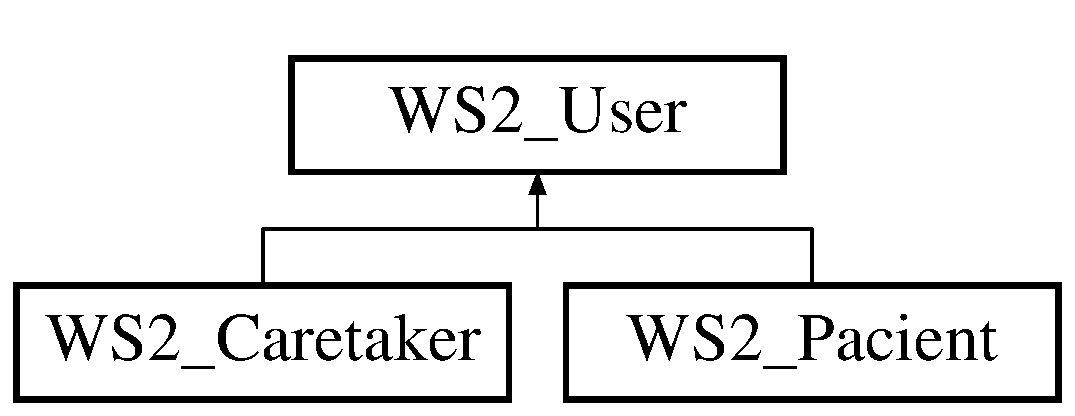
\includegraphics[height=2.000000cm]{class_w_s2___user}
\end{center}
\end{figure}
\subsection*{Public Member Functions}
\begin{DoxyCompactItemize}
\item 
\hypertarget{class_w_s2___user_a42c9621713b6dcdfb9edd5a7630b6d93}{{\bfseries get\+Firstname} ()}\label{class_w_s2___user_a42c9621713b6dcdfb9edd5a7630b6d93}

\item 
\hypertarget{class_w_s2___user_a5d606fdf02d35b79b74b91a88c09000f}{{\bfseries get\+Lastname} ()}\label{class_w_s2___user_a5d606fdf02d35b79b74b91a88c09000f}

\item 
\hypertarget{class_w_s2___user_a81b37a3c9d639574e394f80c1138c75e}{{\bfseries get\+Username} ()}\label{class_w_s2___user_a81b37a3c9d639574e394f80c1138c75e}

\item 
\hypertarget{class_w_s2___user_aeafdb95ad7b97a5ff68ac785e8c243e5}{{\bfseries get\+Birthdate} ()}\label{class_w_s2___user_aeafdb95ad7b97a5ff68ac785e8c243e5}

\item 
\hypertarget{class_w_s2___user_af7313369f22d5c761e16462abe0c6ae1}{{\bfseries get\+Gender} ()}\label{class_w_s2___user_af7313369f22d5c761e16462abe0c6ae1}

\item 
\hypertarget{class_w_s2___user_a211a2979c22afcd7d9056a2bb55aa449}{{\bfseries get\+Token} ()}\label{class_w_s2___user_a211a2979c22afcd7d9056a2bb55aa449}

\item 
\hypertarget{class_w_s2___user_a354f01fe06936133696743e346fc206b}{{\bfseries set\+Token} (\$token)}\label{class_w_s2___user_a354f01fe06936133696743e346fc206b}

\item 
\hyperlink{class_w_s2___user_a718968fc81da151fcdbbdab7bc8e731f}{\+\_\+\+\_\+construct} (\$firstname, \$lastname, \$username, \$birthdate, \$gender)
\end{DoxyCompactItemize}


\subsection{Constructor \& Destructor Documentation}
\hypertarget{class_w_s2___user_a718968fc81da151fcdbbdab7bc8e731f}{\index{W\+S2\+\_\+\+User@{W\+S2\+\_\+\+User}!\+\_\+\+\_\+construct@{\+\_\+\+\_\+construct}}
\index{\+\_\+\+\_\+construct@{\+\_\+\+\_\+construct}!W\+S2\+\_\+\+User@{W\+S2\+\_\+\+User}}
\subsubsection[{\+\_\+\+\_\+construct}]{\setlength{\rightskip}{0pt plus 5cm}\+\_\+\+\_\+construct (
\begin{DoxyParamCaption}
\item[{}]{\$firstname, }
\item[{}]{\$lastname, }
\item[{}]{\$username, }
\item[{}]{\$birthdate, }
\item[{}]{\$gender}
\end{DoxyParamCaption}
)}}\label{class_w_s2___user_a718968fc81da151fcdbbdab7bc8e731f}
constructor for a \hyperlink{class_w_s2___user}{W\+S2\+\_\+\+User}

public \begin{DoxyAuthor}{Author}
firstname and lastname of author, \href{mailto:author@example.org}{\tt author@example.\+org} 
\end{DoxyAuthor}

\begin{DoxyParams}{Parameters}
{\em String} & firstname \\
\hline
{\em String} & lastname \\
\hline
{\em String} & username \\
\hline
{\em String} & birthdate \\
\hline
{\em char} & gender \\
\hline
\end{DoxyParams}


The documentation for this class was generated from the following file\+:\begin{DoxyCompactItemize}
\item 
C\+:/\+Users/\+Alessandro/\+Desktop/\+E\+S-\/\+Project/\+W\+S2/class.\+User.\+php\end{DoxyCompactItemize}

\hypertarget{class_w_s2___webservice}{\section{W\+S2\+\_\+\+Webservice Class Reference}
\label{class_w_s2___webservice}\index{W\+S2\+\_\+\+Webservice@{W\+S2\+\_\+\+Webservice}}
}
\subsection*{Public Member Functions}
\begin{DoxyCompactItemize}
\item 
\hyperlink{class_w_s2___webservice_a94e3fd34f1e7778d69013bc3ac57a1d7}{register\+Pacient} (\$firstname, \$lastname, \$username, \$birthdate, \$gender)
\item 
\hyperlink{class_w_s2___webservice_a3bd4c38e0625889172f441a6c637cc42}{register\+Caretaker} (\$firstname, \$lastname, \$username, \$birthdate, \$gender)
\item 
\hyperlink{class_w_s2___webservice_adb7e6ca2d6bbdfa55a7ccb60c5ce549e}{insert\+Info\+Location} (\$pacient, \$token, \$activity\+Name, \$url)
\item 
\hyperlink{class_w_s2___webservice_ab8824cfa47f27b3ea470c4ceaff1ad99}{authorize\+Caretaker} (\$pacient, \$token, \$activity\+Name, \$caretaker)
\item 
\hyperlink{class_w_s2___webservice_ab93521bcae8c90f705635a5788ce1def}{register\+Method} (\$name\+Method)
\item 
\hypertarget{class_w_s2___webservice_a3c934047380a0debb627d77d51bb85c8}{{\bfseries process\+Request} ()}\label{class_w_s2___webservice_a3c934047380a0debb627d77d51bb85c8}

\end{DoxyCompactItemize}
\subsection*{Data Fields}
\begin{DoxyCompactItemize}
\item 
\hypertarget{class_w_s2___webservice_ad135cc8a47e55f0829949cf62214170f}{{\bfseries \$server} = N\+U\+L\+L}\label{class_w_s2___webservice_ad135cc8a47e55f0829949cf62214170f}

\end{DoxyCompactItemize}


\subsection{Member Function Documentation}
\hypertarget{class_w_s2___webservice_ab8824cfa47f27b3ea470c4ceaff1ad99}{\index{W\+S2\+\_\+\+Webservice@{W\+S2\+\_\+\+Webservice}!authorize\+Caretaker@{authorize\+Caretaker}}
\index{authorize\+Caretaker@{authorize\+Caretaker}!W\+S2\+\_\+\+Webservice@{W\+S2\+\_\+\+Webservice}}
\subsubsection[{authorize\+Caretaker}]{\setlength{\rightskip}{0pt plus 5cm}authorize\+Caretaker (
\begin{DoxyParamCaption}
\item[{}]{\$pacient, }
\item[{}]{\$token, }
\item[{}]{\$activity\+Name, }
\item[{}]{\$caretaker}
\end{DoxyParamCaption}
)}}\label{class_w_s2___webservice_ab8824cfa47f27b3ea470c4ceaff1ad99}
authorize a caretaker to have access to pacient info after validate the pacient, check if the caretaker is in the webservice database and if there's an activity registered. return either a message of error or success

public \begin{DoxyAuthor}{Author}
firstname and lastname of author, \href{mailto:author@example.org}{\tt author@example.\+org} 
\end{DoxyAuthor}

\begin{DoxyParams}{Parameters}
{\em String} & pacient \\
\hline
{\em String} & token \\
\hline
{\em String} & activity\+Name \\
\hline
{\em String} & caretaker \\
\hline
\end{DoxyParams}
\begin{DoxyReturn}{Returns}
String 
\end{DoxyReturn}
\hypertarget{class_w_s2___webservice_adb7e6ca2d6bbdfa55a7ccb60c5ce549e}{\index{W\+S2\+\_\+\+Webservice@{W\+S2\+\_\+\+Webservice}!insert\+Info\+Location@{insert\+Info\+Location}}
\index{insert\+Info\+Location@{insert\+Info\+Location}!W\+S2\+\_\+\+Webservice@{W\+S2\+\_\+\+Webservice}}
\subsubsection[{insert\+Info\+Location}]{\setlength{\rightskip}{0pt plus 5cm}insert\+Info\+Location (
\begin{DoxyParamCaption}
\item[{}]{\$pacient, }
\item[{}]{\$token, }
\item[{}]{\$activity\+Name, }
\item[{}]{\$url}
\end{DoxyParamCaption}
)}}\label{class_w_s2___webservice_adb7e6ca2d6bbdfa55a7ccb60c5ce549e}
insert an pacient activity location after validate its token. return a message of error or success

public \begin{DoxyAuthor}{Author}
firstname and lastname of author, \href{mailto:author@example.org}{\tt author@example.\+org} 
\end{DoxyAuthor}

\begin{DoxyParams}{Parameters}
{\em String} & pacient \\
\hline
{\em String} & token \\
\hline
{\em String} & activity\+Name \\
\hline
{\em String} & url \\
\hline
\end{DoxyParams}
\begin{DoxyReturn}{Returns}
String 
\end{DoxyReturn}
\hypertarget{class_w_s2___webservice_a3bd4c38e0625889172f441a6c637cc42}{\index{W\+S2\+\_\+\+Webservice@{W\+S2\+\_\+\+Webservice}!register\+Caretaker@{register\+Caretaker}}
\index{register\+Caretaker@{register\+Caretaker}!W\+S2\+\_\+\+Webservice@{W\+S2\+\_\+\+Webservice}}
\subsubsection[{register\+Caretaker}]{\setlength{\rightskip}{0pt plus 5cm}register\+Caretaker (
\begin{DoxyParamCaption}
\item[{}]{\$firstname, }
\item[{}]{\$lastname, }
\item[{}]{\$username, }
\item[{}]{\$birthdate, }
\item[{}]{\$gender}
\end{DoxyParamCaption}
)}}\label{class_w_s2___webservice_a3bd4c38e0625889172f441a6c637cc42}
try to register a caretaker, and return either the token or an error message

public \begin{DoxyAuthor}{Author}
firstname and lastname of author, \href{mailto:author@example.org}{\tt author@example.\+org} 
\end{DoxyAuthor}

\begin{DoxyParams}{Parameters}
{\em String} & firstname \\
\hline
{\em String} & lastname \\
\hline
{\em String} & username \\
\hline
{\em String} & birthdate \\
\hline
{\em char} & gender \\
\hline
\end{DoxyParams}
\begin{DoxyReturn}{Returns}
String 
\end{DoxyReturn}
\hypertarget{class_w_s2___webservice_ab93521bcae8c90f705635a5788ce1def}{\index{W\+S2\+\_\+\+Webservice@{W\+S2\+\_\+\+Webservice}!register\+Method@{register\+Method}}
\index{register\+Method@{register\+Method}!W\+S2\+\_\+\+Webservice@{W\+S2\+\_\+\+Webservice}}
\subsubsection[{register\+Method}]{\setlength{\rightskip}{0pt plus 5cm}register\+Method (
\begin{DoxyParamCaption}
\item[{}]{\$name\+Method}
\end{DoxyParamCaption}
)}}\label{class_w_s2___webservice_ab93521bcae8c90f705635a5788ce1def}
Short description of method access\+Info\+Location

public \begin{DoxyAuthor}{Author}
firstname and lastname of author, \href{mailto:author@example.org}{\tt author@example.\+org} 
\end{DoxyAuthor}

\begin{DoxyParams}{Parameters}
{\em String} & caretaker \\
\hline
{\em String} & pacient \\
\hline
{\em String} & activity\+Name \\
\hline
\end{DoxyParams}
\begin{DoxyReturn}{Returns}
W\+S1\+\_\+\+Array 
\end{DoxyReturn}
\hypertarget{class_w_s2___webservice_a94e3fd34f1e7778d69013bc3ac57a1d7}{\index{W\+S2\+\_\+\+Webservice@{W\+S2\+\_\+\+Webservice}!register\+Pacient@{register\+Pacient}}
\index{register\+Pacient@{register\+Pacient}!W\+S2\+\_\+\+Webservice@{W\+S2\+\_\+\+Webservice}}
\subsubsection[{register\+Pacient}]{\setlength{\rightskip}{0pt plus 5cm}register\+Pacient (
\begin{DoxyParamCaption}
\item[{}]{\$firstname, }
\item[{}]{\$lastname, }
\item[{}]{\$username, }
\item[{}]{\$birthdate, }
\item[{}]{\$gender}
\end{DoxyParamCaption}
)}}\label{class_w_s2___webservice_a94e3fd34f1e7778d69013bc3ac57a1d7}
try to register a pacient, and return either the token or an error message

public \begin{DoxyAuthor}{Author}
firstname and lastname of author, \href{mailto:author@example.org}{\tt author@example.\+org} 
\end{DoxyAuthor}

\begin{DoxyParams}{Parameters}
{\em String} & firstname \\
\hline
{\em String} & lastname \\
\hline
{\em String} & username \\
\hline
{\em String} & birthdate \\
\hline
{\em char} & gender \\
\hline
\end{DoxyParams}
\begin{DoxyReturn}{Returns}
String 
\end{DoxyReturn}


The documentation for this class was generated from the following file\+:\begin{DoxyCompactItemize}
\item 
C\+:/\+Users/\+Alessandro/\+Desktop/\+E\+S-\/\+Project/\+W\+S2/class.\+Webservice.\+php\end{DoxyCompactItemize}

%--- End generated contents ---

% Index
\newpage
\phantomsection
\addcontentsline{toc}{chapter}{Index}
\printindex

\end{document}
